\documentclass{article}
\usepackage[utf8]{inputenc}
\usepackage{amsmath}
\usepackage{amsfonts}
\usepackage[margin=0.7in]{geometry}
\usepackage{graphicx}
\usepackage{amssymb}
\usepackage{gensymb}
\usepackage{booktabs}
\usepackage{wrapfig}
\usepackage{caption}
\usepackage[export]{adjustbox}
\usepackage[pdfborder={0 0 0}]{hyperref}
\usepackage{pdfpages}
\usepackage{fancyhdr}
\usepackage{parskip}
\usepackage{lastpage}
\usepackage{listings}
\usepackage{multirow}
\usepackage{xifthen}
\usepackage{xcolor}
\usepackage{mathtools}
\graphicspath{{images/}}
\pagestyle{fancy}

\begin{document}
\title{ØkIntro Aflevering 2}
\author{Carl-Emil Rohde - kvb125}
\date{December 2022}
\maketitle

\section*{Opgave1}
\subsection*{1.1}
Priselasticiteten som funktion af efterspørgsel, også kaldet efterspørgselselasticitet, er givet ved følgende formel:
\begin{equation}
    \epsilon=\frac{p}{q} \frac{dq}{dp}
\end{equation}
Her er $q$ den procentvise ændring i mængden et marked efterspørger, og $p$ er den procentvise ændring i pris. Jeg bruger nu ovenstående formel, på eksemplet i opgaven. 
\\
\\Først indsætter jeg efterspørgselsfunktionen på q's plads:
\begin{equation}
    \epsilon=\frac{p}{B-bp}
\end{equation}
Så ganger jeg $\frac{dq}{dp}$ på, som i det her tilfælde må være $-b$:
\begin{equation}
    \epsilon=\frac{p}{B-bp}*\frac{dq}{dp}=\frac{p}{B-bp}*-b
\end{equation}
Priselasticiteten for efterspørgselsfunktionen, er dermed givet ved: 
\begin{equation}
    \epsilon=\frac{-bp}{B-bp}
\end{equation}

\subsection*{1.2}
For at finde ud af hvad efterspørgelsen skal være, for at opnå en priselasticitet på $-1$, opkriver jeg udtrykket fra forrige opgave, og sætter lig med $-1$:
\begin{equation}
    \frac{-bp}{B-bp}=-1
\end{equation}
Nu isolerer jeg for prisen $p$:
\begin{equation}
    -bp=-1*(B-bp)
\end{equation}
\begin{equation}
    -bp=-B+bp
\end{equation}
\begin{equation}
    -2bp=-B
\end{equation}
\begin{equation}
    p=\frac{-B}{-2b} \Leftrightarrow p=\frac{B}{2b}
\end{equation}
Nu indsætter jeg $p$ i efterspørgselsfunktionen og reducerer:
\begin{equation}
    D(\frac{B}{2b})=B-b(\frac{B}{2b})
\end{equation}
\begin{equation}
    D(\frac{B}{2b})=B-\frac{B}{2} \Leftrightarrow \frac{B}{2}
\end{equation}

Med en priselasticitet på $-1$ er efterspørgslen altså: $\frac{B}{2}$
\\
\\
\\
\subsection*{1.3}
Det første jeg gør, er at finde den inverse efterspørgselsfunktion ved at isolere prisen $p$. Jeg betegner mængden som $q$:
\begin{equation}
    D(p)=B-bp
\end{equation}
\begin{equation}
    p(q)=\frac{B-q}{b}
\end{equation}
For at finde den optimale pris, skal jeg opstille et maksimeringsproblem. Jeg kan spørge, hvilken kvantitet skal virksomheden vælge at sælge, for at maksimere sin profit. Altså: 
\begin{equation}
    MAX_q:\hspace{0.3cm} p(q)*q-c*q
\end{equation}
Her er $p(q)*q$ omsætning, og $c*q$ er omkostninger. 
\\
Jeg indsætter nu $p(q)$ fra den inverse efterspørgselsfunktion i dette udtryk:
\begin{equation}
    MAX_q: \hspace{0.3cm} \frac{B-q}{b} *q-c*q
\end{equation}
Jeg tager nu en førsteordensbetingelse, hvor jeg differentierer ovenstående for $q$. Jeg benytter brøkreglen:
\begin{equation}
    \frac{\partial MAX}{\partial q}(\frac{B-q}{b} *q-c*q) = \frac{B-2q}{b}-c
\end{equation}
I dette udtryk, er $\frac{B-2q}{b}$ vores marginalomsætning, $MR$, og $-c$ er marginalomkostningerne, $MC$. Jeg sætter nu $MR=MC$ og isolerer for $q$:
\begin{equation}
    c=\frac{B-2q}{b}
\end{equation}
\begin{equation}
    bc=B-2q
\end{equation}
\begin{equation}
    2q=bc-B
\end{equation}
\begin{equation}
    q=\frac{bc-B}{2}
\end{equation}
Nu har jeg fundet den optimale mængde. For at finde den tilsvarende optimale pris, kan jeg nu indsætte mit udtryk for $q$, i den inverse efterspørgselsfunktion:

\begin{equation}
    p(q)=\frac{B-q}{b} \Leftrightarrow p(q)=\frac{B-\frac{bc-B}{2}}{b}
\end{equation}
Nu reducerer jeg dette udtrykket:
\begin{equation}
    p(q)=\frac{B}{b}-\frac{\frac{bc-B}{2}}{d}
\end{equation}
\begin{equation}
    p(q)=\frac{B}{b}-\frac{bc-B}{2b}
\end{equation}
\begin{equation}
    p(q)=\frac{2B}{2b}-\frac{bc-B}{2b}
\end{equation}
\begin{equation}
    p(q)=\frac{B-bc}{2b}
\end{equation}
Den optimale pris er dermed givet ved $\frac{B-bc}{2b}$
\\
For at finde ud af, om priselasticiteten er over eller under 1 for den optimale pris, indsætter jeg udtrykket for den optimale pris i formlen for priselasticitet og reducerer:
\begin{equation}
    \epsilon = \frac{-bp}{B-bp}
\end{equation}
\begin{equation}
    \epsilon = \frac{-b*\frac{B-bc}{2b}}{B-b*\frac{B-bc}{2b}}
\end{equation}
\begin{equation}
    \epsilon = \frac{\frac{B-bc}{2b}}{B-\frac{B-bc}{2b}}
\end{equation}
\begin{equation}
    \epsilon = \frac{B+bc}{B-bc}
\end{equation}
Forudsat at $B, b > 0$, vil ovenstående udtryk altid være større end 1, da tælleren er større end nævneren. Priselasticiteten for den optimale pris, er dermed større end 1. 
\\

For at vurdere hvordan den optimale pris, påvirkes af $b$, differentierer jeg den optimale pris, med hensyn til $b$:

\begin{equation}
    \frac{\partial p}{\partial b}= \frac{ \partial \frac{B-bc}{2b}}{\partial b} =\frac{c}{2 b}-\frac{b c+B}{2 b^2}=\frac{B}{2 b^2}
\end{equation}
Det kan her ses, at en stigning i b, medfører et fald i den optimale pris, da nævneren vokser hurtigere end tælleren.

\section*{Opgave 2}
\subsection*{2.1}
Forbrugeren kan både lide forbrug og fritid, men verden fungerer således, at jo mere forbrug man vil have, desto mere fritid må man give afkald på - hvilket også er det skatter til en vis grad påvirker. Jeg vil starte med at opskrive forbrugerens nyttefunktion:
\begin{equation}
    u(c, l)=c-\frac{\eta}{\eta+1}(24-l)^{\frac{\eta+1}{\eta}}
\end{equation}

og opstille et optimeringsproblem under bibetingelse af budgetbetingelsen, som jeg først lige vil omskrive, så jeg isolerer $c$:
\begin{equation}
    pc+wl=24w \Leftrightarrow c+ \frac{w}{p}l=24\frac{w}{p} \Leftrightarrow c=24\frac{w}{p}-\frac{w}{p}l
\end{equation}


på den måde kan jeg finde forbrugrens optimale antal timer at arbejde. Det kommer til at se således ud:
\begin{equation}
    MAX_l=24\frac{w}{p}-\frac{w}{p}l-\frac{\eta}{\eta +1}(24-l)^{\frac{\eta +1}{\eta}} \Leftrightarrow \frac{24 w-l w}{p}-\frac{\eta(-l+24)^{\frac{\eta+1}{\eta}}}{\eta+1}
\end{equation}
Jeg antager at præferencerne er både monotone og konvekse, og opstiller en førsteordensbetingelse, hvor jeg differentierer $\frac{\partial MAX_l}{\partial l}$.
\\
Jeg benytter sumreglen:
\begin{equation}
    \frac{\partial MAX_l}{\partial l} (\frac{24 w-l w}{p}-\frac{\eta(-l+24)^{\frac{\eta+1}{\eta}}}{\eta+1}) = \frac{\partial}{\partial l}\left(\frac{24 w-l w}{p}\right)-\frac{\partial}{\partial l}\left(\frac{\eta(24-l)^{\frac{\eta+1}{\eta}}}{\eta+1}\right) = -\frac{w}{p}-(-(24-l))^{\frac{1}{\eta}}
\end{equation}
ganger fortegn ind og sætter lig 0:
\begin{equation}
    FOB: -\frac{w}{p}+(24-l)^{\frac{1}{\eta}}=0
\end{equation}
Dette kan jeg omskrive til en arbejdsudbudsfunktion af $\frac{w}{p}$:
\begin{equation}
    S(\frac{w}{p})=(24-l)=\frac{w}{p}^{\eta}
\end{equation}
I dette udtryk skal $\eta$ forståes som en arbejdsudbudselasticitet, forstået på den måde at hvis min løn fx stiger med 1 procent, hvor mange flere timer er jeg så villig til at arbejde. $\eta$ er en grundlæggende parameter, når man snakker om hvad den optimale skattesats er.
\\
\\
Med ovenstående udledt, kan jeg nu gå videre med at svare på, hvordan staten maksimerer sine skatteindtægter fra denne arbejder. Obs på, at jeg herfra regner med $p$ som en konstant, $p=1$. Dette antager jeg er ok, da Morten selv gjorde det i forelæsning 7.
\\
\\
Formlen for at udregne skatteprovenue, er givet ved:
\begin{equation}
    T=t*w*s(w(1-t))
\end{equation}
hvor $t*w$ er skat per time, og $s(w(1-t))$ er timer arbejdet. Jeg indsætter nu, det udtryk for optimale antal timer at arbejde jeg fandt før, (hvor $p=1$):
\begin{equation}
    T=t*w*(w(1-t))^{\eta}
\end{equation}
Det jeg har nu, er en funktion for skatteindtægter, også kaldet en lafferkurve. For at finde den optimale skattesats, med henblik på at maksimere statens indtægter, skal jeg finde maksimum for denne kurve. Det vil sige det punkt, hvor den afledte er lig 0.
\\
Jeg differentierer og starter med at bruge konstantregel og dernæst produktregel:
\begin{equation}
    \frac{\partial T}{\partial t}(t*w*(w(1-t))^{\eta}) = w(w(1-t))^{\eta}+tw\eta(w(1-t))^{\eta-1}*(-w) \Leftrightarrow w(w(1-t))^{\eta}-\eta t w^2 (w(1-t))^{\eta -1}
\end{equation}

I dette udtryk, kan $w(w(1-t))^{\eta}$, fortolkes som den positive indvirkning på statens skatteprovenue, da de for hver ekstra time der arbejdes, tjener mere. Dette kaldes også den mekaniske effekt. $-\eta t w^2 (w(1-t))^{\eta -1}$ er derimod et negativt udtryk, og kan fortolkes som en slags adfærdseffekt, der foreskriver at jo hårdere en arbejder bliver beskattet, desto mindre arbejder personen. Når disse to udtryk er lig med hinanden, har vi den optimale skattesats. 
\\
\\
Jeg sætter $\frac{\partial T}{\partial t}=0$ og isolerer for t:
\begin{equation}
    w(w(1-t))^{\eta}-\eta t w^2 (w(1-t))^{\eta -1}=0 \Leftrightarrow w(w(1-t))^{\eta}*(w(1-t))^{-\eta +1}=ntw^2(w(1-t))^{\eta-1}*(w(1-t))^{-\eta+1}
\end{equation}
\begin{equation}
    \Leftrightarrow w(w(1-t))=ntw^2 \Leftrightarrow \frac{w^2(1-t)}{w^2}=\eta t \Leftrightarrow t=\frac{1}{1+\eta}
\end{equation}
Den optimale beskatning for staten, er altså $t=\frac{1}{1+\eta}$

For at finde det højeste skatteprovenue for staten indsætter jeg nu udtrykket for den optimale beskatning, i formlen for skatteprovenue $T=t*w*(w(1-t))^{\eta}$ jeg fandt frem til tidligere:
\begin{equation}
T=\frac{1}{1+\eta} * w *\left(w\left(\frac{1-\frac{1}{1+\eta}}{p}\right)\right)^\eta
\end{equation}
\begin{equation}
    T=\frac{1}{1+\eta} * w *(\frac{(\frac{w*(\eta+1)}{\eta +1})-(\frac{w}{\eta +1})}{p})\eta \Leftrightarrow T=\frac{1}{\eta +1}*w*(\frac{(\frac{w*n}{\eta +1})}{p})^\eta
\end{equation}
Jeg har dermed fundet frem til, hvad det højest mulige skatteprovenue staten kan tjene på Simon er. 
\subsection*{2.2}
Jeg skal finde ud af, om den optimale skattesats jeg fandt i forrige opgave, er for høj til at Tracy gider flytte til Danmark. For at Tracy gider at flytte til Danmark, skal der gælde at hendes nytte efter skat bliver større end højresiden i uligheden:
\begin{equation}
    \Bar{u}>\frac{1}{\eta + 1}(\frac{\eta}{\eta+1}\frac{w}{p})^{\eta +1}
\end{equation}
Jeg får også at vide, at Tracy's nytte er givet ved den samme nyttefunktion som Simon i forrige opgave, altså:
\begin{equation}
    u(c, l)=c-\frac{\eta}{\eta+1}(24-l)^{\frac{\eta+1}{\eta}}
\end{equation}
Jeg går derfor også ud fra, at den optimale skat jeg fandt i forrige opgave, også gælder for Tracy. Jeg kan med det samme se, at udtrykket for $\Bar{u}$, ikke er afhængig af $c$ og $(24-l)$. Derfor opskriver og omskriver jeg Tracy's budgetbetingelse, på samme måde som jeg gjorde med Simon:
\begin{equation}
    pc+wl=24w
\end{equation}
\begin{equation}
    c+ \frac{w}{p}l=24\frac{w}{p}
\end{equation}
\begin{equation}
    c=24\frac{w}{p}-\frac{w}{p}l
\end{equation}
\begin{equation}
    c=\frac{w}{p}(24-l)
\end{equation}
Jeg husker nu, at jeg i forrige opgave da jeg udregnede Simons udbudsfunktion, fandt frem til at $(24-l)=\frac{w}{p}^{\eta}$. Jeg substituerer derfor nu $\frac{w}{p}^{\eta}$ ind i udtrykket:
\begin{equation}
    c=\frac{w}{p}*\frac{w^{\eta}}{p}
\end{equation}
Jeg indsætter nu alt dette i nyttefunktionen:
\begin{equation}
    u=\frac{w}{p}*\frac{w}{p}^{\eta}-\frac{\eta}{\eta+1}((\frac{w}{p})^{\eta})^{\frac{\eta+1}{\eta}}
\end{equation}
Jeg har nu et udtryk der definerer nytten som funktion af arbejdsudbud, i stedet for forbrug og fritis. Jeg reducerer:
\\
\\
Slår brøker sammen:
\begin{equation}
    u=\frac{w}{p}^{1+\eta}-\frac{\eta}{\eta+1}((\frac{w}{p})^{\eta})^{\frac{\eta+1}{\eta}}
\end{equation}
Ganger potenser sammen:
\begin{equation}
    u=\frac{w}{p}^{1+\eta}-\frac{\eta}{\eta-1}(\frac{w}{p})^{\frac{\eta^2+\eta}{\eta}} \Leftrightarrow u=\frac{w}{p}^{1+\eta}-\frac{\eta}{\eta-1}(\frac{w}{p})^{\eta+1}
\end{equation}
Ganger op i tæller og omskriver til brøk:
\begin{equation}
    u=\frac{(\frac{w}{p})^{1+\eta}}{1}-\frac{\eta*(\frac{w}{p})^{\eta+1}}{\eta+1}
\end{equation}
Forlænger den første brøk i udtrykket med $(\eta+1)$:
\begin{equation}
    u=\frac{(\eta+1)*(\frac{w}{p})^{1+\eta}}{(\eta+1)*1}-\frac{\eta*(\frac{w}{p})^{\eta+1}}{\eta+1}
\end{equation}
Laver fælles brøkstreg og ganger paranteser i tælleren ud:
\begin{equation}
    u=\frac{\eta*(\frac{w}{p})^{1+\eta}+(\frac{w}{p})^{1+\eta}-\eta*(\frac{w}{p})^{\eta+1}}{\eta+1}
\end{equation}
$(+/-)\eta*(\frac{w}{p})^{1+\eta}$ går ud med hinanden:
\begin{equation}
    u=\frac{(\frac{w}{p})^{\eta+1
    }}{\eta+1}
\end{equation}
Det næste jeg gør, er at erstatte $w$, altså lønnen før skat, med lønnen efter skat: $w(1-t)$. Derudover, indsætter jeg udtrykket for den optimale skat fra sidste opgave, på $t's$ plads, og reducerer:
\begin{equation}
    u=\frac{(\frac{w(1-\frac{1}{1+\eta})}{p})^{\eta+1
    }}{\eta+1}
\end{equation}
\begin{equation}
    u=\frac{1}{\eta+1}*(\frac{w(1-\frac{1}{1+\eta})}{p})^{\eta+1
    }
\end{equation}
\begin{equation}
    u=\frac{1}{1 + \eta} *\left(\frac{\frac{w \eta}{1+\eta}}{p}\right)^{\eta+1}
\end{equation}
\begin{equation}
u=\frac{1}{\eta+1}\left(\frac{\eta}{1+\eta} \frac{w}{p}\right)^{\eta+1}
\end{equation}
For at det gav mening for Tracy at flytte til Danmark, skulle der gælde at nytten hun fik her, skulle være større, end den fra ulighden i opgavebeskrivelsen. Vi kan nu se, at dette ikke er tilfældet, da nytten hun får i Danmark er lig med og ikke større, end højre side i uligheden. Det er hermed bevist, at den skat der maksimerer skatteprovenuet er “for høj” til at Tracy vil flytte til Danmark.
\subsection*{2.3}
\begin{center}
    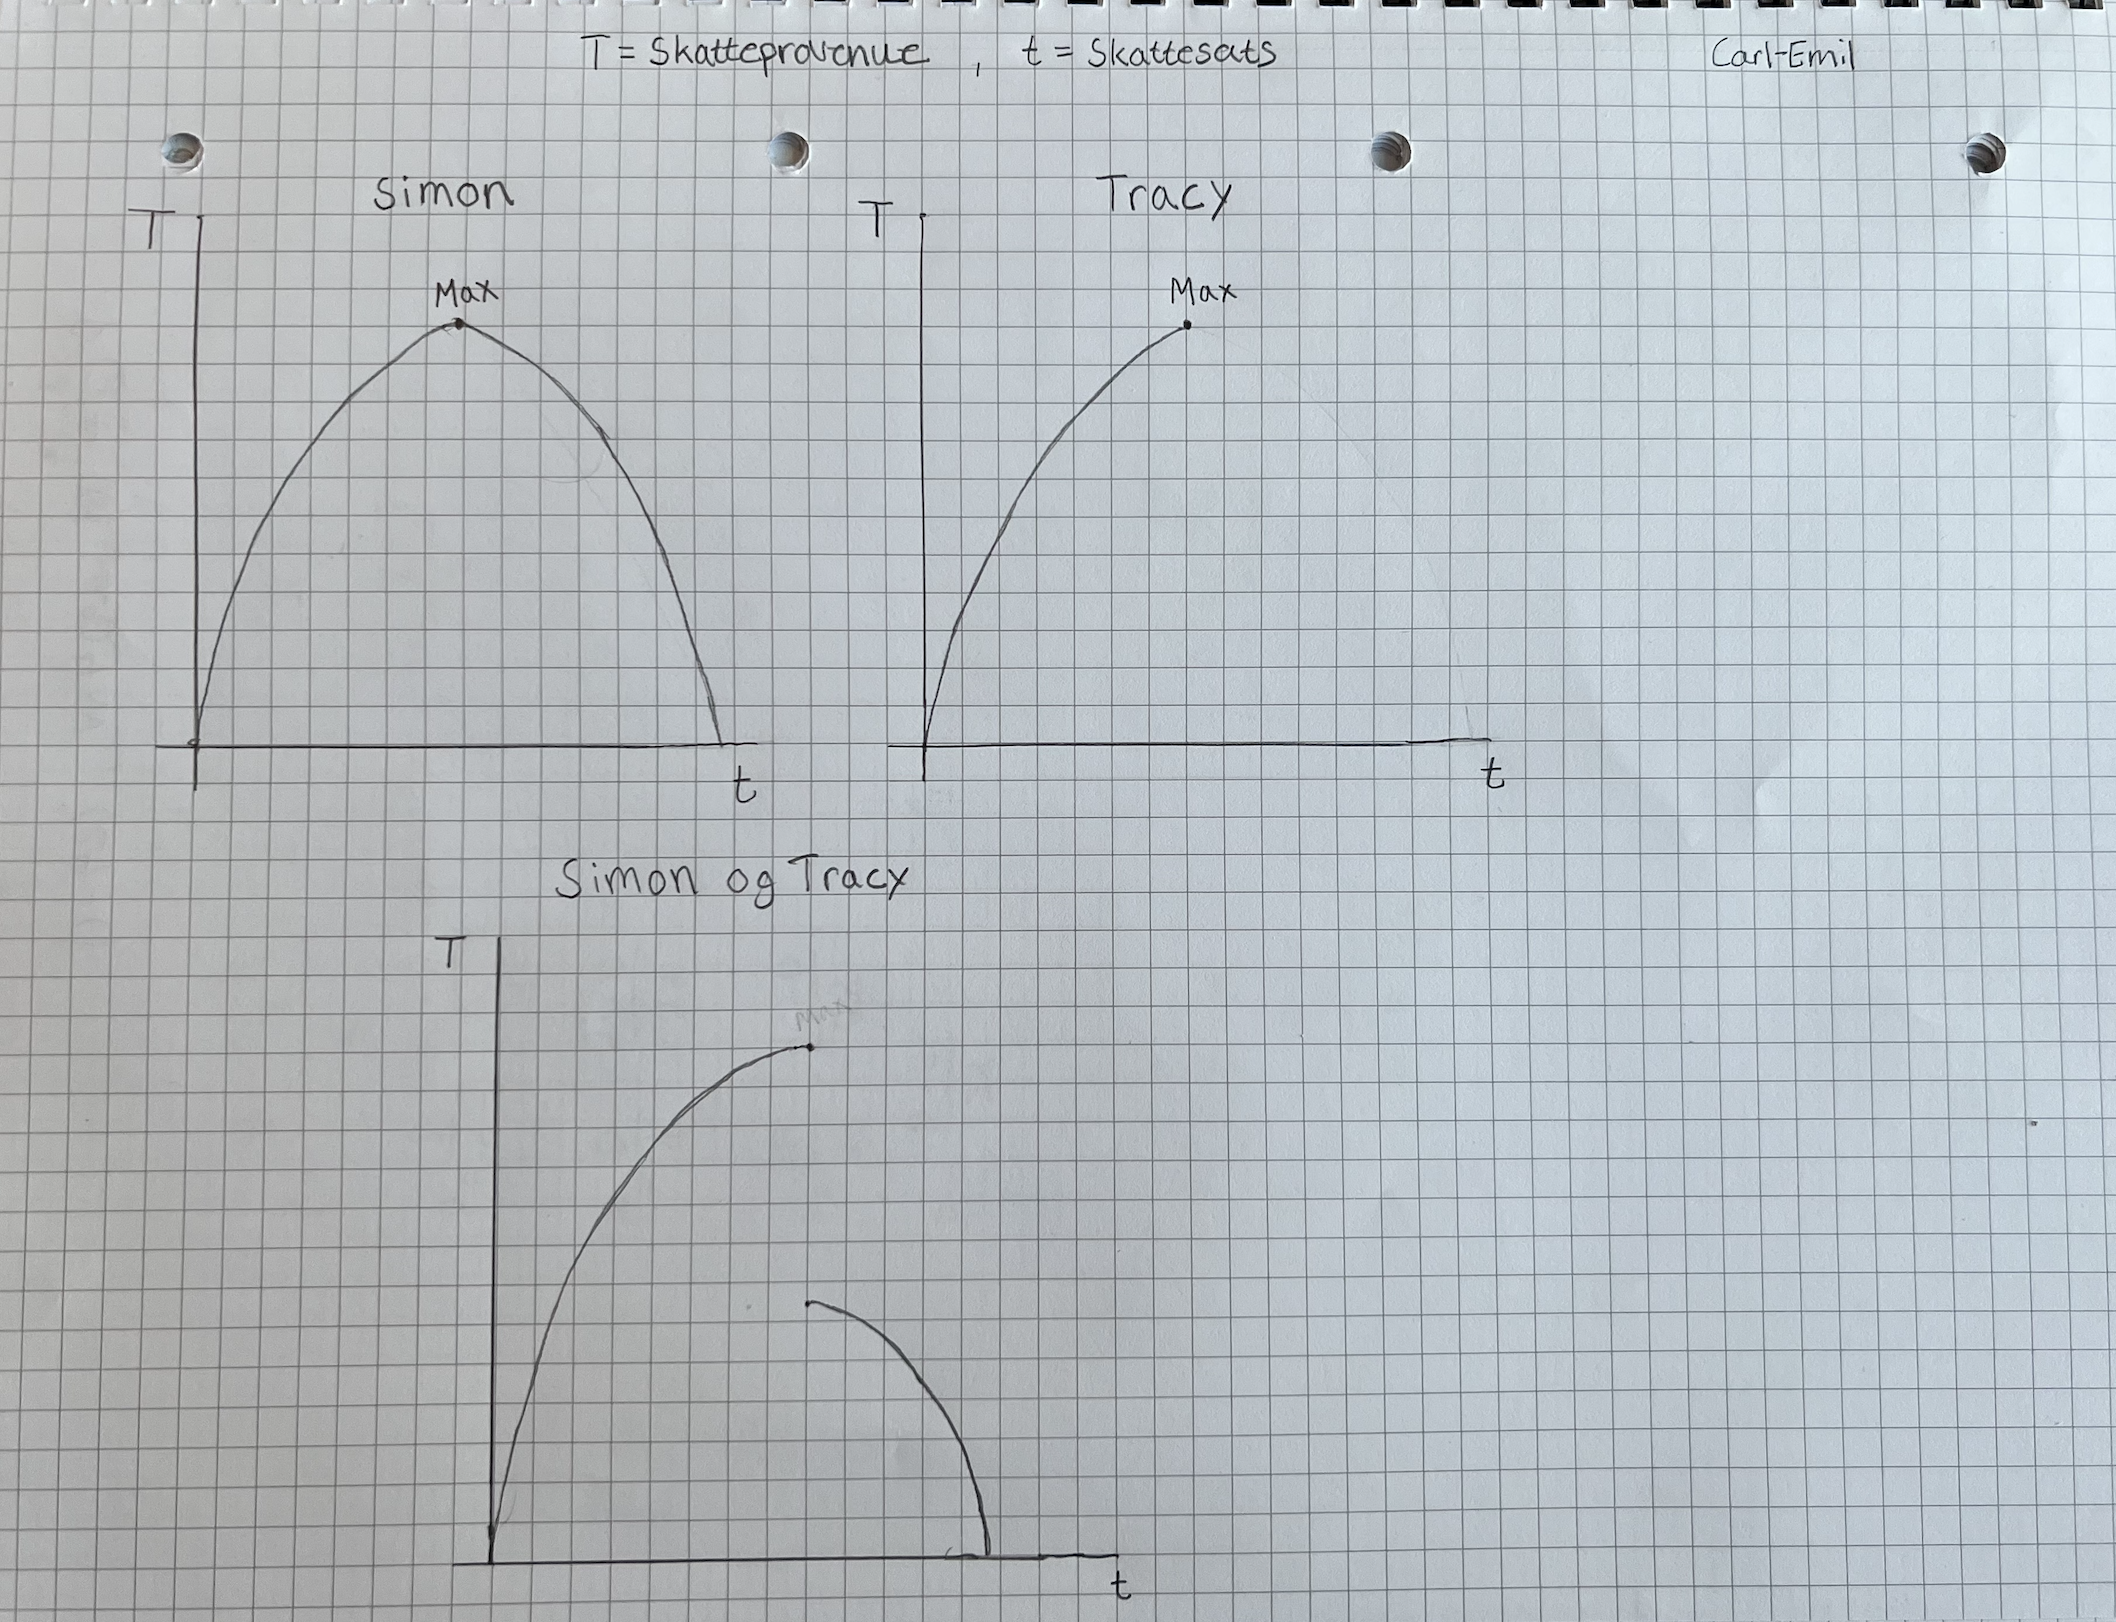
\includegraphics[scale=0.30]{test2.png}
\end{center}
På ovenstående figur, har jeg tegnet både Simon og Tracy's laffer-kurver. Både hver for sig og samlet. Både Simon og Tracy's kurve, har samme toppunkt, da den optimale skattesats for dem begge er den samme. Forskellen er bare, at Tracy jo ikke gider arbejde i Danmark under den optimale skattesats, hvorfor jeg kun har tegnet halvdelen af kurven. Staten tjener altså intet på Tracy, under den optimale skattesats, hvilket også forklarer knækket, i koordinatsystemet hvor jeg har slået kurverne sammen. **Jeg glemte at tegne en lodret streg fra Tracy's $MAX$ og ned til x-aksen**.
\subsection*{2.4}
Problemet ved at sætte én optimal skat for begge forbrugere, altså en uniform skat, er at staten i den situation ikke indkasserer skatteindtægter fra Tracy, som argumenteret for i de forrige opgaver. Ved at lave en differentieret skat (en forskerordning), kan man sætte en optimal skat, der både maksimerer skatteindtægter for Simon og Tracy. Skatten vil i sådan en konstellation være højere for Simon, da han i forvejen er bosat i Danmark - har en stejlere arbejdsudbudskurve, og derfor er villig til at betale mere i skat. Man er derimod nødt til at give Tracy en lavere skat, for at øge hendes incitament til at rejse til Danmark. Dette er grafisk illustreret på bileldet herunder:
\begin{center}
    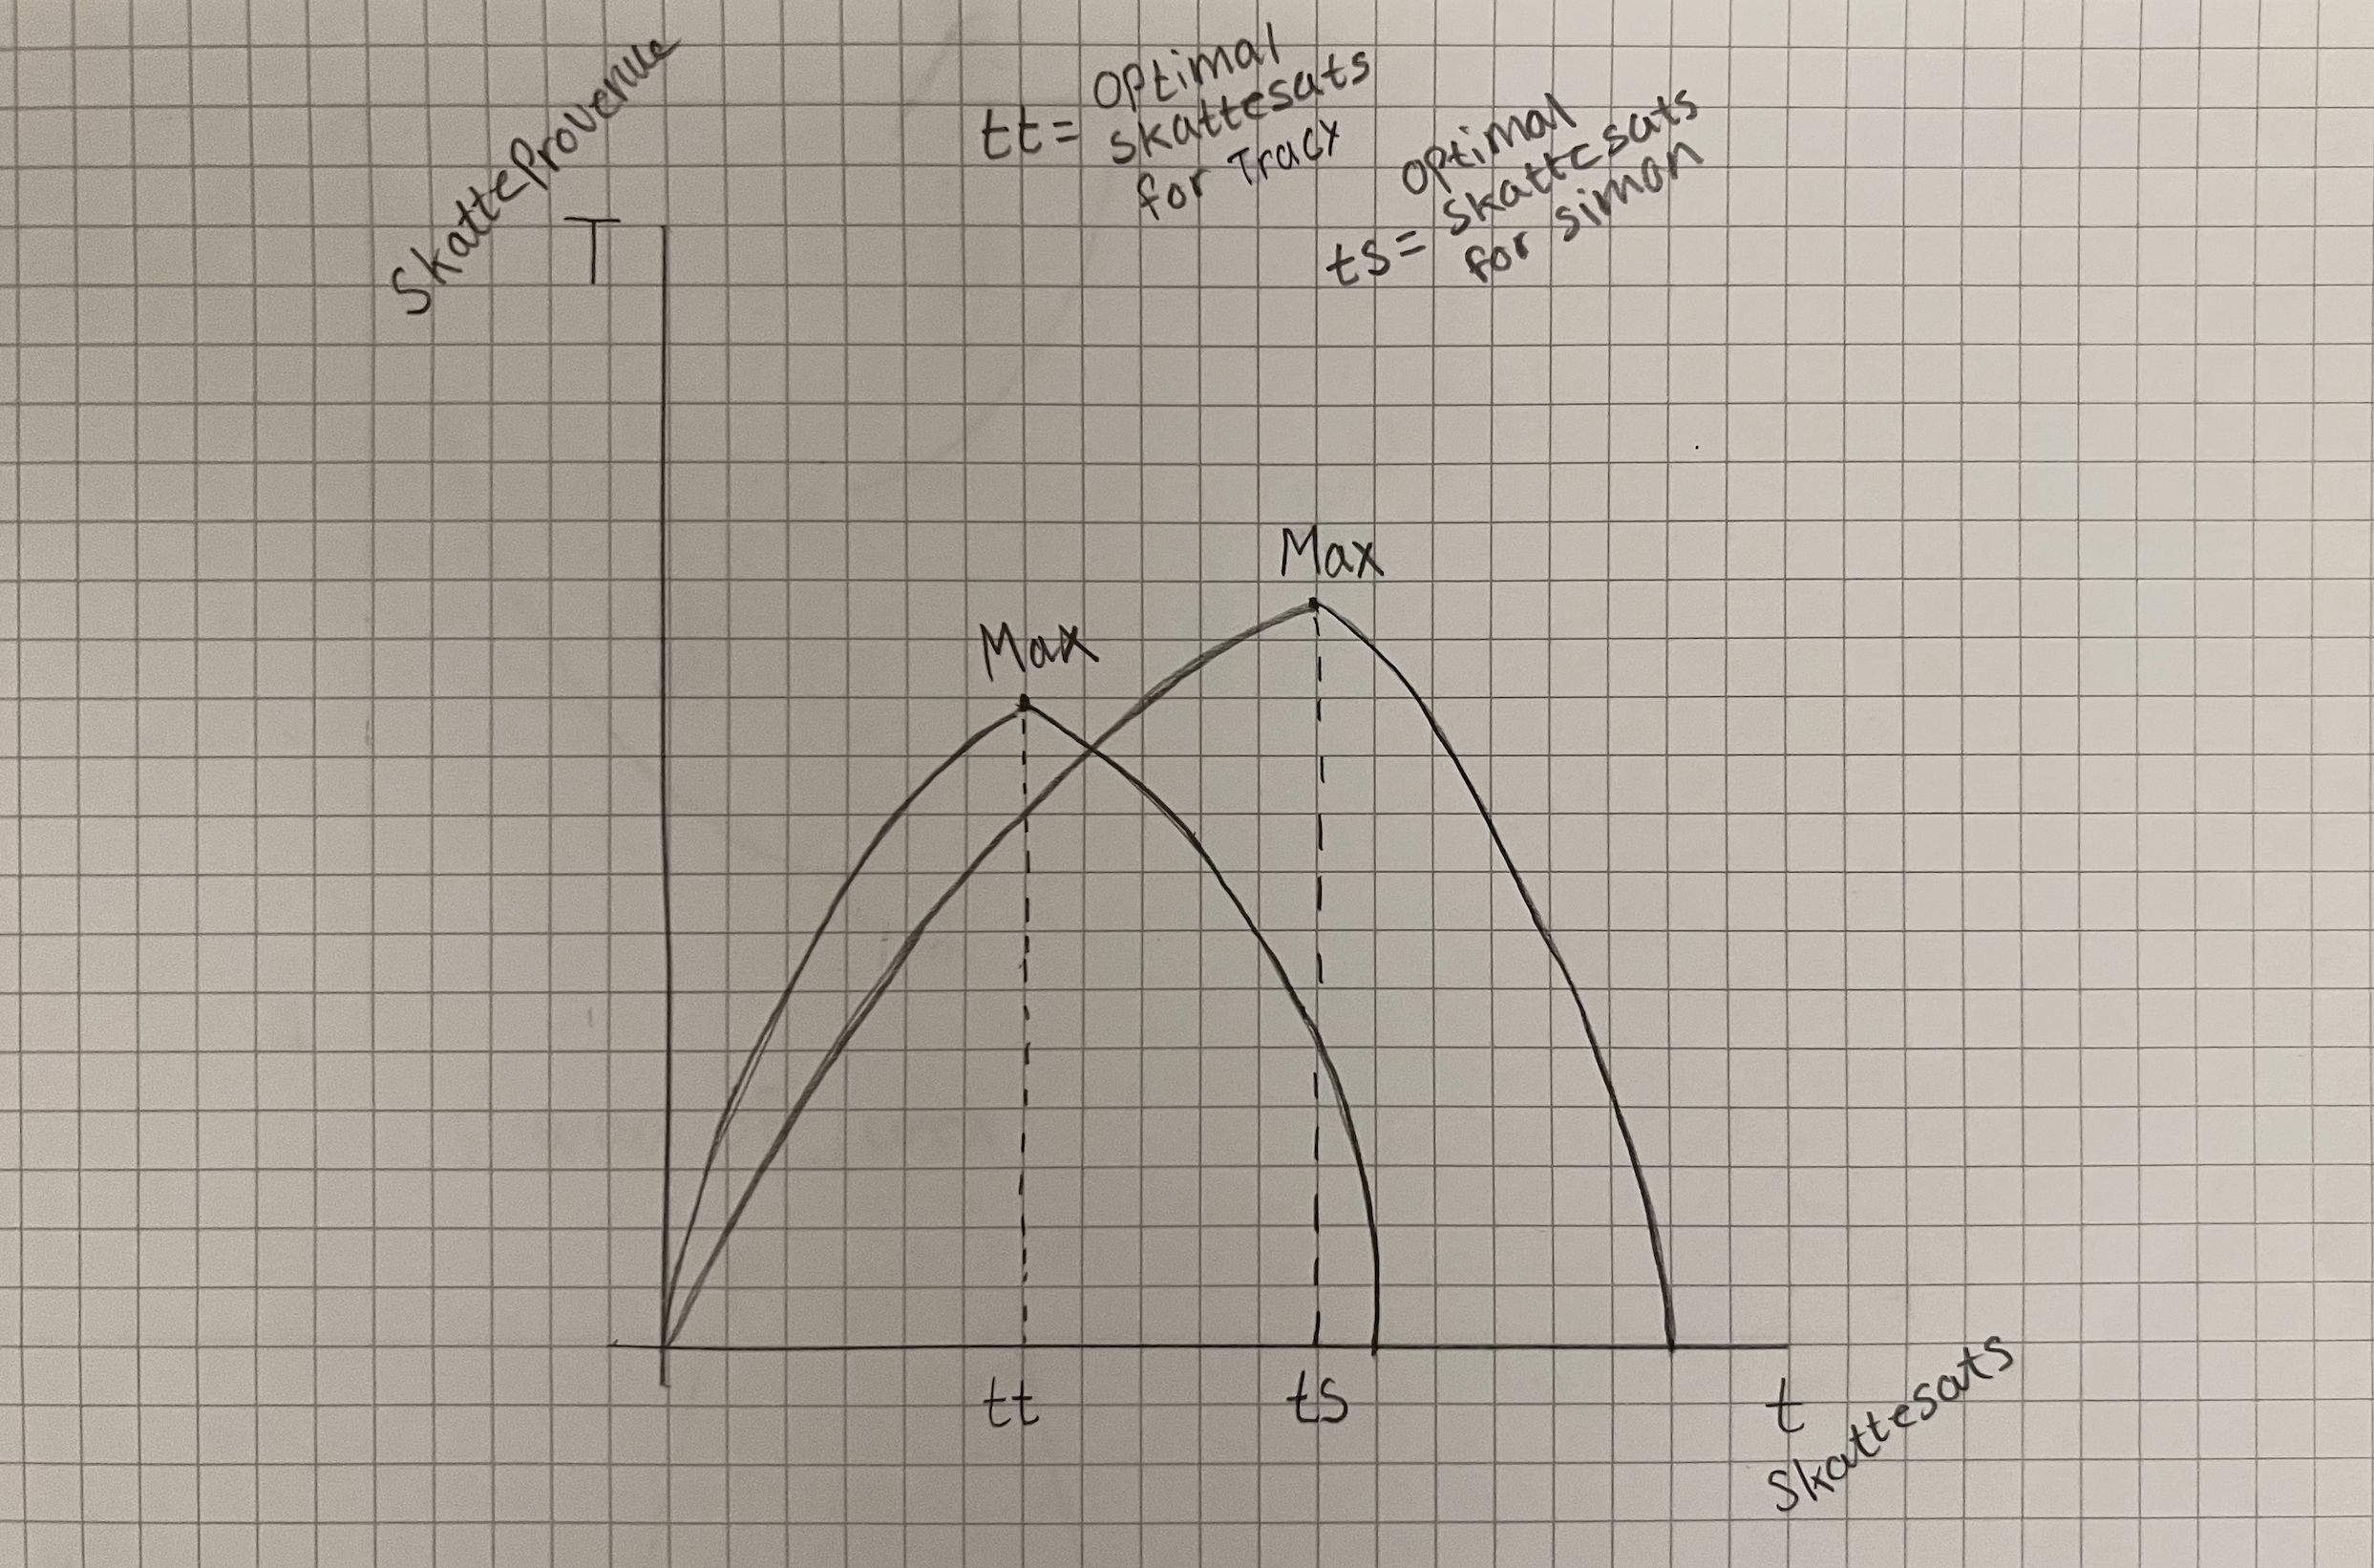
\includegraphics[scale=0.3]{test3.png}
\end{center}
\section*{Opgave 3}
\subsection*{3.1}
Consumer surplus, eller forbrugeroverskuddet er forskellen mellem den pris, en forbruger er villig til at betale for et gode eller en tjeneste, og den faktiske pris, de betaler. Dette overskud kan geometrisk repræsenteres som området under efterspørgselskurven og over markedsligevægtsprisen, altså en trekant. For at udregne arealet af denne trekant, og altså derved consumer surplus, $CS$, sætter jeg først efterspørgselsfunktionen $=0$, og isolerer p:
\begin{equation}
    D(p)=A-ap \Leftrightarrow 0=A-ap
\end{equation}
\begin{equation}
    p=\frac{A}{a}
\end{equation}
Dette udtryk kan fortolkes som det maksimale beløb, forbrugeren er villig til at betale. For at udregne arealet af trekanten, skal jeg selvfølgelig bruge formlen:
\begin{equation}
    A=\frac{1}{2}*højde*grundlinje
\end{equation}
Her bliver højden på trekanten, givet ved forbrugerens maksimale betalingsvillighed (det udtryk for $p$ jeg lige har fundet), minus markedsligevægtsprisen:
\begin{equation}
    \frac{A}{a}-p
\end{equation}
Grundlinjen bliver $A-ap$, og det samlede udtryk ser således sådan ud:
\begin{equation}
    CS=\frac{1}{2}*(\frac{A}{a}-p)*(A-ap) \Leftrightarrow CS=\frac{A^2}{2 a}-A p+\frac{a p^2}{2}
\end{equation}
\subsection*{3.2}
Jeg finder den partielt afledte for $CS$ med hensyn til $p$:
\begin{equation}
    \frac{\partial CS}{\partial p}= (\frac{A^2}{2 a}-A p+\frac{a p^2}{2})
\end{equation}
Jeg bruger sumreglen til at differentiere:
\begin{equation}
    \frac{\partial CS}{\partial p} =(\frac{\partial}{\partial p}\left(\frac{A^2}{2 a}\right)-\frac{\partial}{\partial p}(A p)+\frac{\partial}{\partial p}\left(\frac{a p^2}{2}\right))
\end{equation}
\begin{equation}
    \frac{\partial CS}{\partial p} = 0 - A + ap \Leftrightarrow \frac{\partial CS}{\partial p} = -A+ap
\end{equation}
Ud fra dette resultat, kan det udledes, at en stigning i pris, medfører et fald i efterspørgsel, hvilket også må betyde at Consumer surplus falder. 
\subsection*{3.3}
Jeg finder frem til tabet for forbrugeren, ved at udregne CS igen, men denne gang med skatten inkluderet:
\begin{equation}
    CS=\frac{A^2}{2 a}-A( p+t)+\frac{a (p+t)^2}{2} \Leftrightarrow \frac{A^2}{2 a}-Ap-At+\frac{a (p+t)^2}{2} 
\end{equation}
For at finde tabet for forbrugeren, trækker jeg nu de to udtryk fra hinanden:
\begin{equation}
    \left(\frac{A^2}{2 a}-A p_1+\frac{a p^2}{2}\right)-\left(\frac{A^2}{2 a}-A p_1-A t+\frac{a\left(p+t\right)^2}{2}\right)
\end{equation}
Ganger fortegn ind og deler brøk op:
\begin{equation}
    \frac{A^2}{2a}-Ap+\frac{ap^2}{2}-\frac{A^2}{2a}+Ap+At-\frac{ap^2}{2}-apt-\frac{at^2}{2}
\end{equation}
fjerner led der går ud med hinanden, så tabet for forbrugeren efter skat, altså bliver:
\begin{equation}
    At-apt-\frac{at^2}{2}
\end{equation}
\subsection*{3.4}
Jeg udregner dead weigth loss (DWL), med følgende formel:
\begin{equation}
    DWL=\frac{1}{2}*(p_2-p_1)*(q_2-q_1)
\end{equation}
I mit eksempel er: $p_1=p_1$, $p_2=p_1+t$, $q_1=D(p_1)$ og $q_2=D(p_2)$
Jeg opstiller og reducerer udtrykket:
\begin{equation}
\begin{aligned}
& \text { DWL }=\frac{1}{2} \cdot\left(\left(p_1+t\right)-p_1\right) \cdot\left(D\left(p_1+t\right)-D\left(p_1\right)\right) \\
\end{aligned}
\end{equation}
\begin{equation}
    DWL=\frac{1}{2} \cdot\left(\left(p_1+t\right)-p_1\right) \cdot\left(\left(A-a\left(p_1-t\right)\right)-\left(A-a p_1\right)\right) \\
\end{equation}
\begin{equation}
    DWL= \frac{1}{2} \cdot t\left(-a \cdot\left(p_1+t\right)+a p_1\right) \Rightarrow \frac{1}{2} \cdot t\left(-a p_1-a t+a p_1\right) \\
 \Leftrightarrow \frac{1}{2} \cdot t(-a t) \Leftrightarrow \frac{1}{2} \cdot\left(-a t^2\right) \Leftrightarrow \frac{-a t^2}{2}
\end{equation}
Jeg har altsp fundet $DWL$ til at være $\frac{-at^2}{2}$
\subsection*{3.5}
Jeg starter med at udregne statens provenue. Det gør jeg ved at trække $DWL$ fra forrige opgave, fra forbrugerens tab fra delopgave 3.3:
\begin{equation}
    provenue = (At-apt-\frac{at^2}{2}) - (\frac{-at^2}{2}) = At-apt-a*t^2
\end{equation}
Nu kan jeg sætte $DWL$ over $provenue$:
\begin{equation}
    \frac{DWL}{provenue}=\frac{\frac{at^2}{2}}{At-apt-at^2} = \frac{\frac{at}{2}}{A-apt-at^2} = \frac{\frac{1}{2}at}{A-apt-at^2}
\end{equation}
Her kan vi se, at både $DWL$ og statens provenue afhænger af $a$. Det ses at hvis $a$ vokser, vokser $DWL$ også, da der er en positiv sammenhæng med $a$. $a$ indgår derimod negativt i udtrykket for provenue, hvorfor en stigning i $a$, medfører et fald i statens indtægter. I forholdet mellem de to, er det tydeligt at tælleren vokser hurtigere end nævneren hvis a stiger. Det vil sige forskellen mellem $DWL$ og provenue stiger. En stigning i $a$, svarer til en stigning i efterspørgselselasticiteten. Staten har derfor en interesse i at $a$ ikke bliver for høj, hvis de vil maksimere deres indtægter. 








\end{document}
